\documentclass{standalone}
\usepackage{tikz}
\usetikzlibrary{patterns, positioning}
\usetikzlibrary{shapes.misc}
\usepackage[outline]{contour}
\contourlength{1.5pt} 


\begin{document}
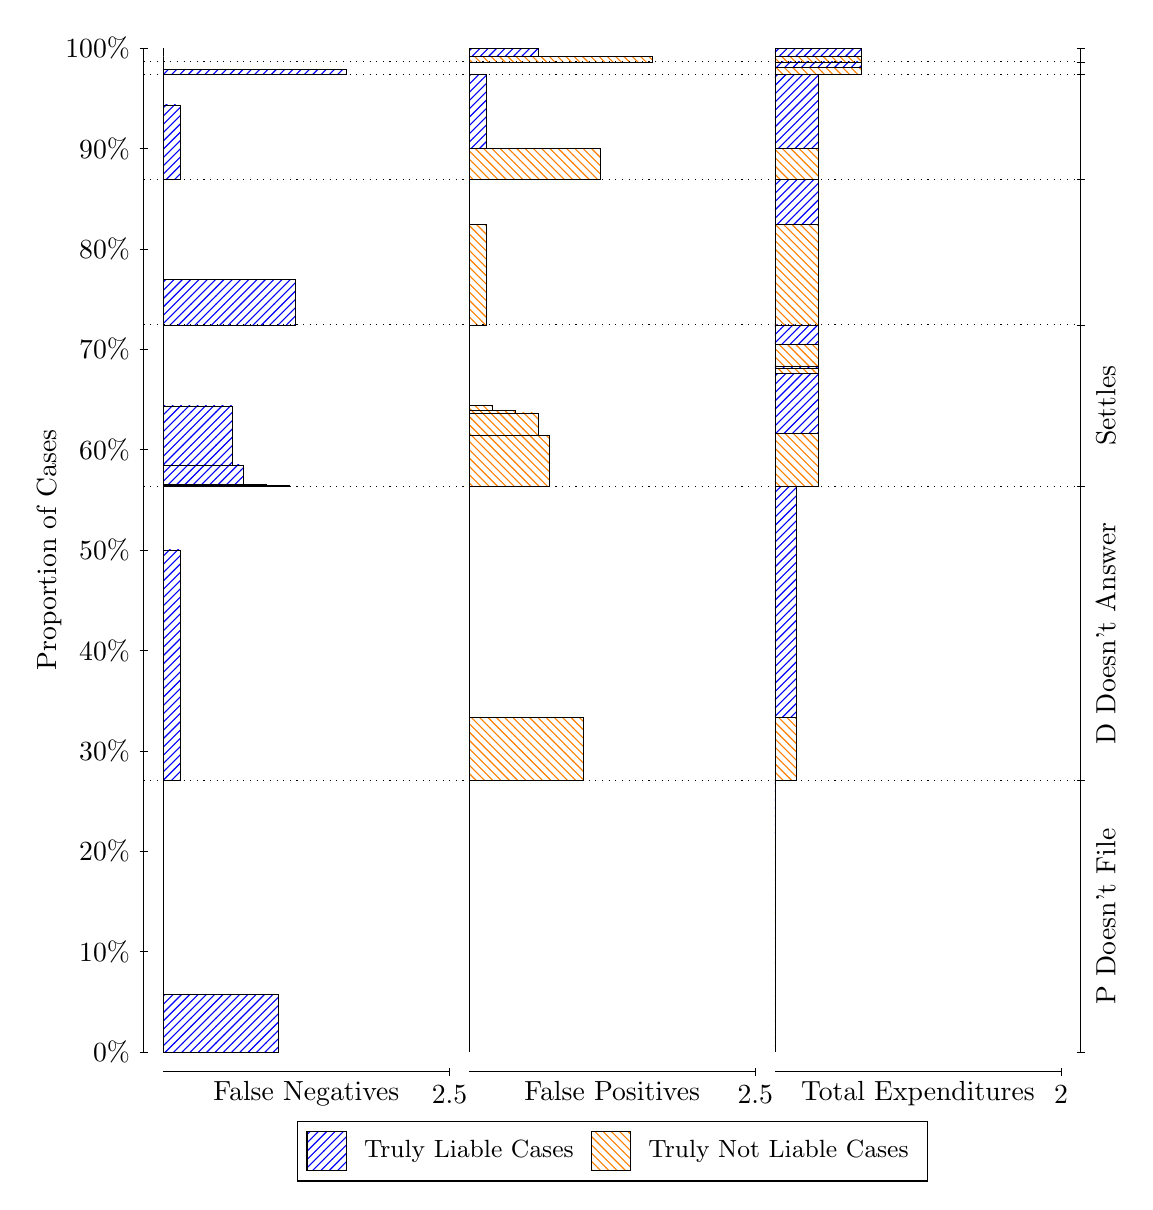
\begin{tikzpicture}
\draw[black, very thin] (1.5,1.75) -- (1.5,14.5);
\node[rotate=90, text=black, anchor=center] at (0.3, 8.125) {Proportion of Cases};
\draw[black, very thin] (1.45,1.75) -- (1.55,1.75);
\node[text=black, anchor=east] at (1.45, 1.75) {0\%};
\draw[black, very thin] (1.45,3.025) -- (1.55,3.025);
\node[text=black, anchor=east] at (1.45, 3.025) {10\%};
\draw[black, very thin] (1.45,4.3) -- (1.55,4.3);
\node[text=black, anchor=east] at (1.45, 4.3) {20\%};
\draw[black, very thin] (1.45,5.575) -- (1.55,5.575);
\node[text=black, anchor=east] at (1.45, 5.575) {30\%};
\draw[black, very thin] (1.45,6.85) -- (1.55,6.85);
\node[text=black, anchor=east] at (1.45, 6.85) {40\%};
\draw[black, very thin] (1.45,8.125) -- (1.55,8.125);
\node[text=black, anchor=east] at (1.45, 8.125) {50\%};
\draw[black, very thin] (1.45,9.4) -- (1.55,9.4);
\node[text=black, anchor=east] at (1.45, 9.4) {60\%};
\draw[black, very thin] (1.45,10.675) -- (1.55,10.675);
\node[text=black, anchor=east] at (1.45, 10.675) {70\%};
\draw[black, very thin] (1.45,11.95) -- (1.55,11.95);
\node[text=black, anchor=east] at (1.45, 11.95) {80\%};
\draw[black, very thin] (1.45,13.225) -- (1.55,13.225);
\node[text=black, anchor=east] at (1.45, 13.225) {90\%};
\draw[black, very thin] (1.45,14.5) -- (1.55,14.5);
\node[text=black, anchor=east] at (1.45, 14.5) {100\%};

\draw[black, very thin] (13.4,1.75) -- (13.4,14.5);
\draw[black, very thin] (13.35,1.75) -- (13.45,1.75);
\node[anchor=west] at (13.35, 1.75) {};
\draw[black, very thin] (13.35,5.1944) -- (13.45,5.1944);
\node[anchor=west] at (13.35, 5.1944) {};
\draw[black, very thin] (13.35,8.9325) -- (13.45,8.9325);
\node[anchor=west] at (13.35, 8.9325) {};
\draw[black, very thin] (13.35,10.984) -- (13.45,10.984);
\node[anchor=west] at (13.35, 10.984) {};
\draw[black, very thin] (13.35,12.835) -- (13.45,12.835);
\node[anchor=west] at (13.35, 12.835) {};
\draw[black, very thin] (13.35,14.166) -- (13.45,14.166);
\node[anchor=west] at (13.35, 14.166) {};
\draw[black, very thin] (13.35,14.324) -- (13.45,14.324);
\node[anchor=west] at (13.35, 14.324) {};
\draw[black, very thin] (13.35,14.5) -- (13.45,14.5);
\node[anchor=west] at (13.35, 14.5) {};

\draw[black, very thin, pattern color=blue, pattern=north east lines] (1.75,1.75) rectangle (3.2033,2.479);
\draw[black, very thin, pattern color=orange, pattern=north west lines] (1.75,2.479) rectangle (1.75,5.1944);
\draw[black, very thin, pattern color=blue, pattern=north east lines] (1.75,5.1944) rectangle (1.968,8.127);
\draw[black, very thin, pattern color=orange, pattern=north west lines] (1.75,8.127) rectangle (1.75,8.9325);
\draw[black, very thin, pattern color=blue, pattern=north east lines] (1.75,8.9325) rectangle (3.3487,8.9494);
\draw[black, very thin, pattern color=blue, pattern=north east lines] (1.75,8.9494) rectangle (3.058,8.9628);
\draw[black, very thin, pattern color=blue, pattern=north east lines] (1.75,8.9628) rectangle (2.7673,9.2063);
\draw[black, very thin, pattern color=blue, pattern=north east lines] (1.75,9.2063) rectangle (2.622,9.9552);
\draw[black, very thin, pattern color=orange, pattern=north west lines] (1.75,9.9552) rectangle (1.75,10.984);
\draw[black, very thin, pattern color=blue, pattern=north east lines] (1.75,10.984) rectangle (3.4213,11.56);
\draw[black, very thin, pattern color=orange, pattern=north west lines] (1.75,11.56) rectangle (1.75,12.835);
\draw[black, very thin, pattern color=blue, pattern=north east lines] (1.75,12.835) rectangle (1.968,13.777);
\draw[black, very thin, pattern color=orange, pattern=north west lines] (1.75,13.777) rectangle (1.75,14.166);
\draw[black, very thin, pattern color=blue, pattern=north east lines] (1.75,14.166) rectangle (4.0753,14.233);
\draw[black, very thin, pattern color=orange, pattern=north west lines] (1.75,14.233) rectangle (1.75,14.324);
\draw[black, very thin, pattern color=orange, pattern=north west lines] (1.75,14.324) rectangle (1.75,14.394);
\draw[black, very thin, pattern color=blue, pattern=north east lines] (1.75,14.394) rectangle (1.75,14.5);
\draw[black, very thin, pattern color=orange, pattern=north west lines] (5.6333,1.75) rectangle (5.6333,4.4654);
\draw[black, very thin, pattern color=blue, pattern=north east lines] (5.6333,4.4654) rectangle (5.6333,5.1944);
\draw[black, very thin, pattern color=orange, pattern=north west lines] (5.6333,5.1944) rectangle (7.0867,6);
\draw[black, very thin, pattern color=blue, pattern=north east lines] (5.6333,6) rectangle (5.6333,8.9325);
\draw[black, very thin, pattern color=orange, pattern=north west lines] (5.6333,8.9325) rectangle (6.6507,9.5782);
\draw[black, very thin, pattern color=orange, pattern=north west lines] (5.6333,9.5782) rectangle (6.5053,9.8669);
\draw[black, very thin, pattern color=orange, pattern=north west lines] (5.6333,9.8669) rectangle (6.2147,9.8937);
\draw[black, very thin, pattern color=orange, pattern=north west lines] (5.6333,9.8937) rectangle (5.924,9.9615);
\draw[black, very thin, pattern color=blue, pattern=north east lines] (5.6333,9.9615) rectangle (5.6333,10.984);
\draw[black, very thin, pattern color=orange, pattern=north west lines] (5.6333,10.984) rectangle (5.8513,12.26);
\draw[black, very thin, pattern color=blue, pattern=north east lines] (5.6333,12.26) rectangle (5.6333,12.835);
\draw[black, very thin, pattern color=orange, pattern=north west lines] (5.6333,12.835) rectangle (7.3047,13.224);
\draw[black, very thin, pattern color=blue, pattern=north east lines] (5.6333,13.224) rectangle (5.8513,14.166);
\draw[black, very thin, pattern color=orange, pattern=north west lines] (5.6333,14.166) rectangle (5.6333,14.257);
\draw[black, very thin, pattern color=blue, pattern=north east lines] (5.6333,14.257) rectangle (5.6333,14.324);
\draw[black, very thin, pattern color=orange, pattern=north west lines] (5.6333,14.324) rectangle (7.9587,14.394);
\draw[black, very thin, pattern color=blue, pattern=north east lines] (5.6333,14.394) rectangle (6.5053,14.5);
\draw[black, very thin, pattern color=orange, pattern=north west lines] (9.5167,1.75) rectangle (9.5167,4.4654);
\draw[black, very thin, pattern color=blue, pattern=north east lines] (9.5167,4.4654) rectangle (9.5167,5.1944);
\draw[black, very thin, pattern color=orange, pattern=north west lines] (9.5167,5.1944) rectangle (9.7892,6);
\draw[black, very thin, pattern color=blue, pattern=north east lines] (9.5167,6) rectangle (9.7892,8.9325);
\draw[black, very thin, pattern color=orange, pattern=north west lines] (9.5167,8.9325) rectangle (10.062,9.605);
\draw[black, very thin, pattern color=blue, pattern=north east lines] (9.5167,9.605) rectangle (10.062,10.367);
\draw[black, very thin, pattern color=orange, pattern=north west lines] (9.5167,10.367) rectangle (10.062,10.435);
\draw[black, very thin, pattern color=blue, pattern=north east lines] (9.5167,10.435) rectangle (10.062,10.452);
\draw[black, very thin, pattern color=orange, pattern=north west lines] (9.5167,10.452) rectangle (10.062,10.741);
\draw[black, very thin, pattern color=blue, pattern=north east lines] (9.5167,10.741) rectangle (10.062,10.984);
\draw[black, very thin, pattern color=orange, pattern=north west lines] (9.5167,10.984) rectangle (10.062,12.26);
\draw[black, very thin, pattern color=blue, pattern=north east lines] (9.5167,12.26) rectangle (10.062,12.835);
\draw[black, very thin, pattern color=orange, pattern=north west lines] (9.5167,12.835) rectangle (10.062,13.224);
\draw[black, very thin, pattern color=blue, pattern=north east lines] (9.5167,13.224) rectangle (10.062,14.166);
\draw[black, very thin, pattern color=orange, pattern=north west lines] (9.5167,14.166) rectangle (10.607,14.257);
\draw[black, very thin, pattern color=blue, pattern=north east lines] (9.5167,14.257) rectangle (10.607,14.324);
\draw[black, very thin, pattern color=orange, pattern=north west lines] (9.5167,14.324) rectangle (10.607,14.394);
\draw[black, very thin, pattern color=blue, pattern=north east lines] (9.5167,14.394) rectangle (10.607,14.5);
\draw[black, dotted] (1.5,5.1944) -- (13.4,5.1944);
\draw[black, dotted] (1.5,8.9325) -- (13.4,8.9325);
\draw[black, dotted] (1.5,10.984) -- (13.4,10.984);
\draw[black, dotted] (1.5,12.835) -- (13.4,12.835);
\draw[black, dotted] (1.5,14.166) -- (13.4,14.166);
\draw[black, dotted] (1.5,14.324) -- (13.4,14.324);
\draw[black, very thin] (1.75,1.5) -- (5.3833,1.5);
\node[text=black, anchor=north] at (3.5667, 1.5) {False Negatives};
\draw[black, very thin] (5.3833,1.45) -- (5.3833,1.55);
\node[text=black, anchor=north] at (5.3833, 1.45) {2.5};

\draw[black, very thin] (5.6333,1.5) -- (9.2667,1.5);
\node[text=black, anchor=north] at (7.45, 1.5) {False Positives};
\draw[black, very thin] (9.2667,1.45) -- (9.2667,1.55);
\node[text=black, anchor=north] at (9.2667, 1.45) {2.5};

\draw[black, very thin] (9.5167,1.5) -- (13.15,1.5);
\node[text=black, anchor=north] at (11.333, 1.5) {Total Expenditures};
\draw[black, very thin] (13.15,1.45) -- (13.15,1.55);
\node[text=black, anchor=north] at (13.15, 1.45) {2};

\node[text=black, centered, rotate=90] at (13.72, 3.4722) {\contour{white}{P Doesn't File}};
\node[text=black, centered, rotate=90] at (13.72, 7.0635) {\contour{white}{D Doesn't Answer}};
\node[text=black, centered, rotate=90] at (13.72, 9.9584) {\contour{white}{Settles}};





\draw (7.449999999999999,1.5) node[draw=none] (baseCoordinate) {};
\begin{scope}[align=center]
        \matrix[scale=0.5, draw=black, below=0.5cm of baseCoordinate, nodes={draw}, column sep=0.1cm]{
            \node[rectangle, draw, minimum width=0.5cm, minimum height=0.5cm, pattern color=blue, pattern=north east lines] {}; &
            \node[draw=none, font=\small, text=black] (B) {Truly Liable Cases}; &
            \node[rectangle, draw, minimum width=0.5cm, minimum height=0.5cm, pattern color=orange, pattern=north west lines] {}; &
            \node[draw=none, font=\small, text=black] (B) {Truly Not Liable Cases}; \\
            };
\end{scope}

\end{tikzpicture}
\end{document}